\documentclass{article}
\usepackage[a4paper]{geometry}
\usepackage[T1]{fontenc}
\usepackage[utf8]{inputenc}
\usepackage[italian]{babel}
\usepackage{geometry}
\usepackage[font={small,sl}]{caption}
\usepackage[section]{placeins}
\usepackage{graphicx}
\usepackage[table, dvipsnames]{xcolor}
\usepackage{subcaption}
\usepackage{listings}
\usepackage{fancyhdr}
\usepackage{amssymb}
\usepackage{amsmath}
\usepackage[font={small,sl}]{caption}
\usepackage{hyperref}

\def\code#1{\texttt{#1}}

\setlength{\parskip}{1em}
\setlength{\parindent}{0em}
\setlength{\arrayrulewidth}{0.1em}

\hypersetup{
    colorlinks=true,
    citecolor=blue,
    linkcolor=blue,
    linktocpage=true,
    urlcolor=blue,
    pdftitle={Relazione Progetto SOA},
    pdfauthor={C. Cuffaro}
}

% Colori per i listing
\definecolor{code_red}{rgb}{0.6,0,0} % strings
\definecolor{code_green}{rgb}{0.25,0.5,0.35} % comments
\definecolor{code_purple}{rgb}{0.5,0,0.35} % keywords
\definecolor{code_background}{rgb}{0.95,0.95,0.92} % background

% Stile del codice standard (C)
\lstset{
	language=C, 
	backgroundcolor=\color{code_background},
	frame=single,
	basicstyle=\ttfamily\small,
	keywordstyle=\color{code_purple}\bfseries\small,
	stringstyle=\color{code_red}\small,
	commentstyle=\color{code_green}\small,
	numbers=left,
	numberstyle=\small\color{gray},
	numbersep=5pt,
	tabsize=4,
	showtabs=false,
	showspaces=false,
	showstringspaces=false,
	escapechar=|, 
	captionpos=b,
	breaklines=true,
}

\renewcommand{\lstlistingname}{Snippet}

\pagestyle{fancy}
\fancyhf{}
\lhead{\small C. Cuffaro}
\rhead{\small Relazione Progetto SOA}
\cfoot{\thepage}
%\cfoot{Pagina \thepage}

\begin{document}
\author{%
Cristiano Cuffaro \\
{\small matricola: \texttt{0299838}} \\
{\small \texttt{cristiano.cuffaro@outlook.com}}
}
\title{Relazione Progetto SOA}
\date{A.A. 2021-2022}

\maketitle
\tableofcontents
\newpage

\section{Rappresentazione dei device file}
In accordo alla specifica del progetto e ai casi d'uso che si possono derivare da essa, è stata scelta una rappresentazione in RAM per i \textsl{multi-flow device file}.

In particolare, uno stream di dati è implementato come una \textsl{linked list} di segmenti di dati dinamicamente allocati e agganciati tra una \textsl{head} ed una \textsl{tail} fittizie, come mostrato nella rappresentazione in figura \ref{fig-1}.

\captionsetup[figure]{justification=centering}
\begin{figure}[ht]
\centering
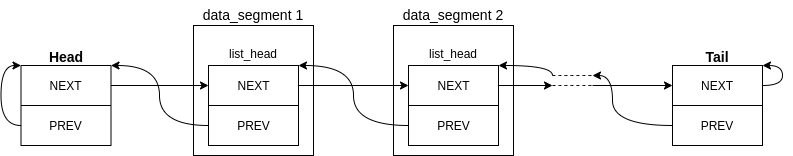
\includegraphics[width=0.8\textwidth]{img/segment-list}
\caption{Lista di segmenti che implementa un data stream}
\label{fig-1}
\end{figure}

Per ciascun segmento di dati, all'interno di una struttura \texttt{data\_segment} sono mantenute le seguenti informazioni:
\begin{itemize}
\item un puntatore ai dati effettivi;
\item la dimensione corrente dei dati;
\item un indice che rappresenta la posizione corrente di lettura;
\item una struttura \texttt{list\_head} per il collegamento alla lista.
\end{itemize}
Quando è necessario allocare un nuovo segmento di dati, avviene un'unica chiamata verso lo \textsl{SLAB allocator} per ottenere un'area di memoria in cui impaccare la struttura dati nella parte alta e i dati effettivi in quella bassa. Inoltre, per limitare la dimensione reale della struttura a 40 byte è stata definita specificando l'attributo \texttt{packed}.

In una struttura \texttt{device\_struct} sono definite le informazioni associate a ciascun device, in particolare:
\begin{itemize}
\item una waitqueue per ciascun data stream, ove si tiene traccia dei thread in attesa di prelevare o scaricare dati nel caso di letture o scritture bloccanti;
\item una workqueue per mantenere il lavoro da eseguire in maniera \textsl{delayed} nel caso di scritture a bassa priorità;
\item un mutex per ciascun data stream, necessario per sincronizzare le operazioni di lettura e scrittura;
\item una struttura \texttt{segment\_list} per ciascun data stream, contenente gli elementi fittizi della lista;
\item il numero di byte validi in ciascun data stream, ovvero quelli effettivamente leggibili;
\item il numero di byte liberi in ciascun data stream, ovvero quelli che determinano la possibilità di eseguire delle operazioni di scrittura;
\item il numero di thread in attesa di dati per ciascun data stream, ovvero la cardinalità dell'insieme dei lettori all'interno della corrispondente waitqueue.
\end{itemize}
Per aumentare il livello di sicurezza del VFS, per questa struttura dati è stata utilizzata la dicitura \texttt{\_\_randomize\_layout}, in modo tale che un eventuale attacco finalizzato a prelevare informazioni da un device file sia ostacolato dal fatto che lo spiazzamento a cui sono presenti i dati è arbitrario e cambia tra i vari kernel.

Nella funzione di inizializzazione del modulo non vengono create workqueue standard, bensì \textsl{singlethread workqueue}. Questo fa sì che il deferred work sia processato lungo un unico \textsl{kworker deamon}, che riporta le operazioni di scrittura sul data stream di bassa priorità nello stesso ordine con cui sono state schedulate, senza necessità di meccanismi di ordinamento o sincronizzazione ulteriori.

\section{Operazioni sui multi-flow device file}
Nelle seguenti sottosezioni sono descritte le funzioni che costituiscono il driver, ovvero che permettono di eseguire le varie operazioni sui device file che esso gestisce.

\subsection{Operazione di apertura}
La funzione \texttt{mfd\_open} consente l'apertura di un multi-flow device file. Ad ogni invocazione, essa verifica che il minor number associato al dispositivo sia gestibile dal driver e che esso non sia correntemente disabilitato. Se i controlli vanno a buon fine, viene allocata la memoria per ospitare una struttura \texttt{session\_data} contenente le seguenti informazioni:
\begin{itemize}
\item il livello di priorità dello stream di dati su cui si sta correntemente lavorando (bassa priorità per default);
\item l'intervallo di tempo che determina la massima attesa per le operazioni di lettura e scrittura bloccanti (10 secondi per default).
\end{itemize}
Per mantenere il puntatore a questa struttura viene sfruttato il campo \texttt{.private\_data} della struttura \texttt{file} corrispondente alla sessione di I/O.

Per determinare se l'operazione di apertura è stata eseguita in modalità non bloccante, viene controllato se all'interno del campo \texttt{file->f\_flags} è settato il flag \texttt{O\_NONBLOCK}. In caso di operazioni non bloccanti, tutte le allocazioni di memoria vengono eseguite specificando la maschera \texttt{GFP\_ATOMIC}, grazie alla quale la chiamata verso l'allocatore di memoria può fallire senza portare il thread a dormire qualora non vi fosse memoria immediatamente disponibile.

\subsection{Operazione di rilascio}
La funzione \texttt{mfd\_release} è invocata quando viene rilasciata la struttura \texttt{file} e, in maniera duale rispetto alla \texttt{mfd\_open}, si occupa di riconsegnare all'allocatore l'area di memoria puntata da \texttt{file->private\_data}.

\subsection{Operazione di lettura}
La funzione \texttt{mfd\_read} viene invocata quando si esegue un'operazione di lettura su un multi-flow device file.

Se per la sessione di I/O è settato il flag \texttt{O\_NONBLOCK}, viene fatto quanto segue:
\begin{enumerate}
\item si esegue una trylock sul mutex relativo allo stream di dati da cui si vuole leggere;
\item si verifica se la quantità di dati leggibili è pari a zero;
\end{enumerate}
se fallisce l'acquisizione del mutex o non ci sono dati da leggere, la funzione restituisce \texttt{-EAGAIN}.

Se l'operazione di lettura è eseguita in modalità bloccante, si procede come segue:
\begin{enumerate}
\item viene incrementato il numero di thread in attesa di dati provenienti dal data stream in questione;
\item viene invocata l'API \texttt{wait\_event\_interruptible\_timeout} specificando:
\begin{enumerate}
\item la waitqueue corrispondente al data stream;
\item la condizione che determina il risveglio dei thread;
\item il timeout presente tra i dati di sessione;
\end{enumerate}
\item se il thread esce dal sonno per via del termine del timeout o per una segnalazione, la funzione restituisce l'errore corrispondente.
\end{enumerate}
Per far sì che ogni \textsl{wake up} porti al risveglio di al più un thread posto sulla waitqueue, invece di specificare direttamente alla wait queue API la condizione che il numero di byte leggibili sia maggiore di zero, viene specificata la macro \texttt{lock\_and\_check}, mostrata nello snippet \ref{lst-1}.
\begin{lstlisting}[label=lst-1, caption={Macro \texttt{lock\_and\_check}}]
#define lock_and_check(condition, mutexp)       \
({                                              \
        int __ret = 0;                          \
        if (mutex_trylock(mutexp)) {            \
                if (condition)                  \
                        __ret = 1;              \
                else                            \
                        mutex_unlock(mutexp);   \
        }                                       \
        __ret;                                  \
})
\end{lstlisting}
Grazie ad essa, è possibile provare ad acquisire il lock prima di controllare la condizione reale su cui eventualmente dormire; per cui un solo thread ha la possibilità di risvegliarsi avendo già acquisito il lock, se la condizione è soddisfatta. In tutti gli altri casi il valore della macro sarà zero e i thread torneranno a dormire.

Una volta usciti dalla \texttt{wait\_event\_interruptible\_timeout}, si decrementa il numero di thread in attesa e si prosegue con la lettura effettiva dei dati.

Sia nel caso di operazione bloccante che non, una volta acquisito il lock la lettura effettiva è realizzata invocando la funzione \texttt{actual\_read} in cui si cerca di copiare tutto (o in parte) l'ammontare di byte indicato dall'utente all'interno del buffer specificato. Per farlo, dovendo rispettare una politica di consegna FIFO, vengono letti i segmenti di dati a partire dalla testa della lista, facendone avanzare l'indice di lettura ed eventualmente rimuovendoli non appena vuotati. Questa operazione altera sia il numero di byte validi per il data stream (riducendolo), che quello di byte liberi (incrementandolo).

Al termine dell'operazione di lettura (o a valle di un errore riscontrato eseguendo la sezione critica) viene eseguita l'API \texttt{wake\_up\_interruptible} per segnalare ad eventuali thread dormienti di verificare la condizione per la quale sono in attesa e infine viene restituito il numero di byte consegnati nel buffer utente (o l'opportuno codice d'errore).

\subsection{Operazione di scrittura}
La funzione \texttt{mfd\_write} viene invocata quando si esegue un'operazione di scrittura su un multi-flow device file.

Prima di acquisire il lock, viene allocata la memoria per il nuovo segmento di dati che dovrà essere collegato alla lista corrispondente al data stream su cui si sta lavorando; ciò consentirà di acquisire e rilasciare il lock nel minor tempo possibile. Sia nel caso di operazione bloccante che non, per poter eseguire la sezione critica viene svolto lo stesso lavoro analizzato per l'operazione di lettura, con la differenza che la condizione che consente di eseguire la scrittura è che il numero di byte liberi sia maggiore di zero. Per osservare un blocco in scrittura, è necessario che la dimensione dello stream di dati raggiunga il valore \texttt{MAX\_STRAM\_SIZE}, che per default è stato definito pari a \texttt{4*PAGE\_SIZE}.

Una volta acquisito il lock, se l'operazione di scrittura ha come target il data stream ad alta priorità, deve essere eseguita in maniera sincrona e quindi viene invocata la funzione \texttt{actual\_write} che collega il segmento di dati in coda alla lista. In questo caso, anche questa operazione altera sia il numero di byte validi per il data stream (incrementandolo), che quello di byte liberi (riducendolo).

Se l'operazione è invece a bassa priorità deve essere eseguita in maniera asincrona e quindi è necessario programmarne l'esecuzione. A tale scopo, prima di acquisire il lock viene allocata memoria anche per una struttura \texttt{packed\_write} che embedda quella da inserire nella workqueue, contenente le seguenti informazioni:
\begin{itemize}
\item la \texttt{work\_struct} effettiva;
\item il minor number del device su cui andare a scrivere;
\item il puntatore al segmento di dati da agganciare;
\item il function pointer che porta al blocco di codice che esegue la reale operazione.
\end{itemize}
Per cui, la scrittura a bassa priorità si riduce all'invocazione di \texttt{schedule\_deferred\_work}, in cui:
\begin{enumerate}
\item viene eseguita una invocazione a \texttt{try\_module\_get} per incrementare lo \texttt{usage counter} del modulo ed evitare che possa essere smontato mentre c'è ancora del lavoro da svolgere nonostante non vi siano più sessioni verso i multi-flow device file;
\item viene inizializzata la \texttt{work\_struct} indicando la \texttt{deferred\_write} come funzione che il kworker deamon dorvà eseguire e passando l'indirizzo della struttura stessa come dato;
\item viene messo in coda il lavoro.
\end{enumerate}
Fatto ciò, viene decrementato solamente il numero di byte liberi, in modo tale che le altre operazioni di lettura e scrittura non siano compromesse dal fatto che un segmento di dati verrà agganciato in un istante successivo alla sua schedulazione.

A questo livello di priorità, la reale operazione di scrittura verrà invocata dal kworker deamon che eseguirà la funzione \texttt{deferred\_write}, in cui:
\begin{enumerate}
\item all'indirizzo della struttura \texttt{work\_struct}, passato come argomento, viene applicata la macro \texttt{to\_packed\_write} che semplicemente utilizza \texttt{container\_of} per ottenere l'indirizzo della struttura \texttt{packed\_write} contenente le informazioni necessarie alla funzione per operare;
\item viene invocata la funzione \texttt{actual\_write} che collega il segmento di dati in coda alla lista e a questo punto incrementa anche il numero di byte validi per il data stream;
\item viene eseguita l'API \texttt{wake\_up\_interruptible};
\item viene rilasciata la memoria che ospitava la struttura dati \texttt{packed\_write};
\item viene decrementato lo usage counter del modulo.
\end{enumerate}

Sia nel caso di operazione di scrittura sincrona che asincrona, il valore di ritorno di \texttt{mfd\_write} è dato dal numero di byte (eventualmente inferiore a quello specificato dall'utente) che sono stati prelevati dallo user space, indipendentemente da quando questi verranno resi realmente disponibili.

\subsection{Operazione di I/O control}
La funzione \texttt{mfd\_ioctl} viene invocata quando si esegue una richiesta di gestione di un multi-flow device file.

Di seguito sono descritte le richieste di \textsl{I/O control} che vengono gestite.
\begin{itemize}
\item \texttt{IOC\_SWITCH\_PRIORITY}, permette di cambiare il livello di priorità (alto o basso) con cui verranno eseguite le successive operazioni di lettura e scrittura per la sessione corrente;
\item \texttt{IOC\_SWITCH\_BLOCKING}, permette di cambiare il valore del flag \texttt{O\_NONBLOCK} e di conseguenza far sì che le successive operazioni di lettura e scrittura siano eseguite in modalità bloccante o non per la sessione corrente;
\item \texttt{IOC\_SET\_WAIT\_TIMEINT}, permette di impostare il massimo intervallo di tempo di attesa, espresso in secondi, per le operazioni di lettura e scrittura bloccanti.
\end{itemize}

L'aggiunta di questa ioctl è stata fatta utilizzando le convenzionali \texttt{\_IO} macro, che sono basate su una lettera o un numero che identifica il driver per le quali vengono utilizzate. In questo caso, la scelta sul cosiddetto \textsl{IOCTL magic number} e sui numeri associati alle singole macro è stata fatta evitando collisioni con le informazioni presenti nella tabella reperibile al seguente link:
\begin{center}
\url{https://www.kernel.org/doc/Documentation/ioctl/ioctl-number.txt}
\end{center}

\section{Parametri del modulo}
Per rappresentare lo stato di operatività dei multi-flow device file, è stata utilizzata una variabile globale \texttt{device\_status} definita come parametro mediante la macro \texttt{module\_param\_array}. In questo modo è possibile sfruttare lo pseudo-file presente in \texttt{/sys} per abilitare o disabilitare un multi-flow device file.

Per offrire le altre informazioni richieste come parametri non è stato seguito lo stesso approccio e questo ha evitato di duplicare le informazioni già presenti nella struttura dati \texttt{device\_struct} all'interno di variabili globali. In particolare, per ottenere una soluzione alternativa è stato osservato che all'interno della macro \texttt{module\_param\_array\_named} sono utilizzate le seguenti variabili:
\begin{itemize}
\item \texttt{param\_array\_ops}, che è la struttura \texttt{kernel\_param\_ops} contenente i function pointer verso le operazioni di \texttt{get}, \texttt{set} e \texttt{free} da eseguire quando si interagisce con un parametro che consiste in un array;
\item \texttt{param\_ops\_\#\#type}, che è anch'essa una struttura \texttt{kernel\_param\_ops} il cui indirizzo viene assegnato al campo \texttt{.ops} di una struttura \texttt{kparam\_array} per indicare il set di operazioni da eseguire su ciascuna entry di tipo \texttt{type} del parametro.
\end{itemize}
Poiché nel kernel Linux le funzioni registrate in \texttt{param\_array\_ops} non sono state esportate (e.g. \texttt{param\_array\_get}), non è stato possibile definire una sorta di \textsl{wrapper} che a seconda del parametro su cui si sta lavorando può assumere un comportamento differente da quello standard. Per cui, la soluzione adottata è stata quella di definire una nuova macro \texttt{mfd\_module\_param\_array\_named} nella quale si utilizzano:
\begin{itemize}
\item \texttt{mfd\_param\_array\_ops}, in cui è registrata la sola funzione \texttt{mfd\_param\_array\_get} che viene invocata quando si cerca di listare il contenuto dello pseudo-file corrispondente al parametro.

Internamente, per ogni entry dell'array invoca la funzione registrata nel campo \texttt{ops->get} della struttura \texttt{kparam\_array}, passando come argomento l'indice della entry stessa e ciò permette di determinare il contenuto della corrispondente riga dello pseudo-file;

\item \texttt{mfd\_param\_ops\_\#\#type}, dove nel caso specifico si ha che \texttt{\#\#type} corrisponde sempre a \texttt{charp} e anche qui è stata registrata la sola funzione \texttt{mfd\_param\_get\_charp}, che a seconda del nome del parametro:
\begin{itemize}
\item produce una rappresentazione in caratteri del numero di byte presenti su ciascun data stream;
\item produce una rappresentazione in caratteri del numero di thread in attesa di dati da ciascun data stream;
\item in altri casi si comporta per default come l'originale \texttt{param\_get\_charp}.
\end{itemize}
Come specificato nel bullet precedente, nel campo \texttt{arg} della struttura \texttt{kernel\_param} è possibile reperire l'indice della entry per cui questa funzione sta eseguendo e questo coincide con il minor number del dispositivo, per cui si possono leggere le informazioni richieste direttamente dalla corrispondente struttura dati.
\end{itemize}

\section{Struttura del progetto}
Di seguito è riportata un'indicazione dei file sorgenti ed header presenti all'interno della root directory del progetto.
\begin{itemize}
\item \texttt{docs/}
\begin{itemize}
\item \texttt{drawio/} è la cartella contenente gli schemi costruiti su \url{https://app.diagrams.net/}.
\item \texttt{img/} è la cartella contenente le immagini della relazione.
\item \texttt{relazione.pdf} è il documento corrente.
\end{itemize}
\item \texttt{include/}
\begin{itemize}
\item \texttt{ioctl.h} è il file header in cui sono definiti i comandi per poter eseguire richieste di I/O control.
\item \texttt{mfd.h} è il file header in cui sono definite le macro, le strutture dati e le funzioni \textsl{inline} a supporto del modulo.
\end{itemize}
\item \texttt{Makefile}
\item \texttt{multi-flowdev.c} è il file sorgente principale per il modulo del kernel Linux che è stato sviluppato.
\item \texttt{README.md}
\item \texttt{user/}
\begin{itemize}
\item \texttt{device-controller.c} è un \textsl{thin client} molto semplice che può essere utilizzato per testare il funzionamento del driver.
\end{itemize}
\end{itemize}

\section{Regole di compilazione}
Posizionandosi nella root directory del progetto è possibile eseguire una o più delle seguenti regole di compilazione:
\begin{itemize}
\item \texttt{make [all]}
\begin{itemize}
\item compila la versione di base del modulo
\end{itemize}
\item \texttt{make debug}
\begin{itemize}
\item compila la versione del modulo predisposta per eseguirne il debug, poiché definisce il flag \texttt{DEBUG} che attiva le stampe di livello kernel eseguite con l'API \texttt{pr\_debug}
\end{itemize}
\item \texttt{make single-session}
\begin{itemize}
\item compila la versione del modulo in cui per ciascun device è presente un ulteriore mutex che ne consente l'uso esclusivo ed è pensato per un profilo operazionale in cui c'è la necessità di scrivere, in maniera temporalmente discontinua, una sequenza di dati logicamente continua
\end{itemize}
\item \texttt{make clean}
\begin{itemize}
\item elimina i file generati dalla compilazione
\end{itemize}
\item \texttt{make disable DEV=<minor>}
\begin{itemize}
\item consente di disabilitare il multi-flow device file corrispondente al minor number specificato
\end{itemize}
\item \texttt{make enable DEV=<minor>}
\begin{itemize}
\item consente di abilitare il multi-flow device file corrispondente al minor number specificato
\end{itemize}
\end{itemize}

Per generare il file eseguibile corrispondente al thin client è sufficiente:
\begin{enumerate}
\item posizionarsi all'interno della directory \texttt{user/}
\item eseguire il comando \texttt{make}
\end{enumerate}
e per la sua esecuzione:
\begin{center}
\texttt{./device-controller <NodePath> <Major> <Minor>}
\end{center}

\end{document}